% !TeX root = ../../Skript.tex
\cohead{\Large\textbf{Wendepunkte}}
\fakesubsection{Wendepunkte}
Als Wendepunkte bezeichnet man die Punkte des Schaubilds einer Funktion an denen die Krümmung wechselt, also das Schaubild von einer Linkskurve in eine Rechtskurve übergeht oder umgekehrt. Anders ausgedrückt, das Schaubild einer Funktion hat genau dann einen Wendepunkt, wenn die zweite Ableitung eine Nullstelle mit Vorzeichenwechsel hat.\\
Die folgenden drei Aussagen sind äquivalent:

\bigskip

\begin{minipage}{\textwidth}
	\adjustbox{valign=t}{\begin{minipage}{\textwidth/\real{3}-1ex}
		\begin{tcolorbox}[width=\textwidth, height=4cm, valign=center]
			\textcolor{loestc}{Das Schaubild von \(f(x)\) hat bei \(x_0\) einen Wendepunkt.}
		\end{tcolorbox}\end{minipage}}%
	\adjustbox{valign=t, padding=1.5ex 0ex 0ex 0ex}{\begin{minipage}{\textwidth/\real{3}-1ex}
		\begin{tcolorbox}[width=\textwidth, height=4cm, valign=center]
			\textcolor{loestc}{Das Schaubild von \(f'(x)\) hat bei \(x_0\) einen Extrempunkt.}
		\end{tcolorbox}\end{minipage}}%
	\adjustbox{valign=t, padding=1.5ex 0ex 0ex 0ex}{\begin{minipage}{\textwidth/\real{3}-1ex}
		\begin{tcolorbox}[width=\textwidth, height=4cm, valign=center]
			\textcolor{loestc}{Das Schaubild von \(f''(x)\) hat bei \(x_0\) eine Nullstelle mit Vorzeichenwechsel.}
		\end{tcolorbox}\end{minipage}}%
\end{minipage}

\bigskip

Beispiel:

\bigskip

\begin{minipage}{\textwidth}
	\adjustbox{valign=t}{\begin{minipage}{\textwidth/\real{3}-1ex}
			\centering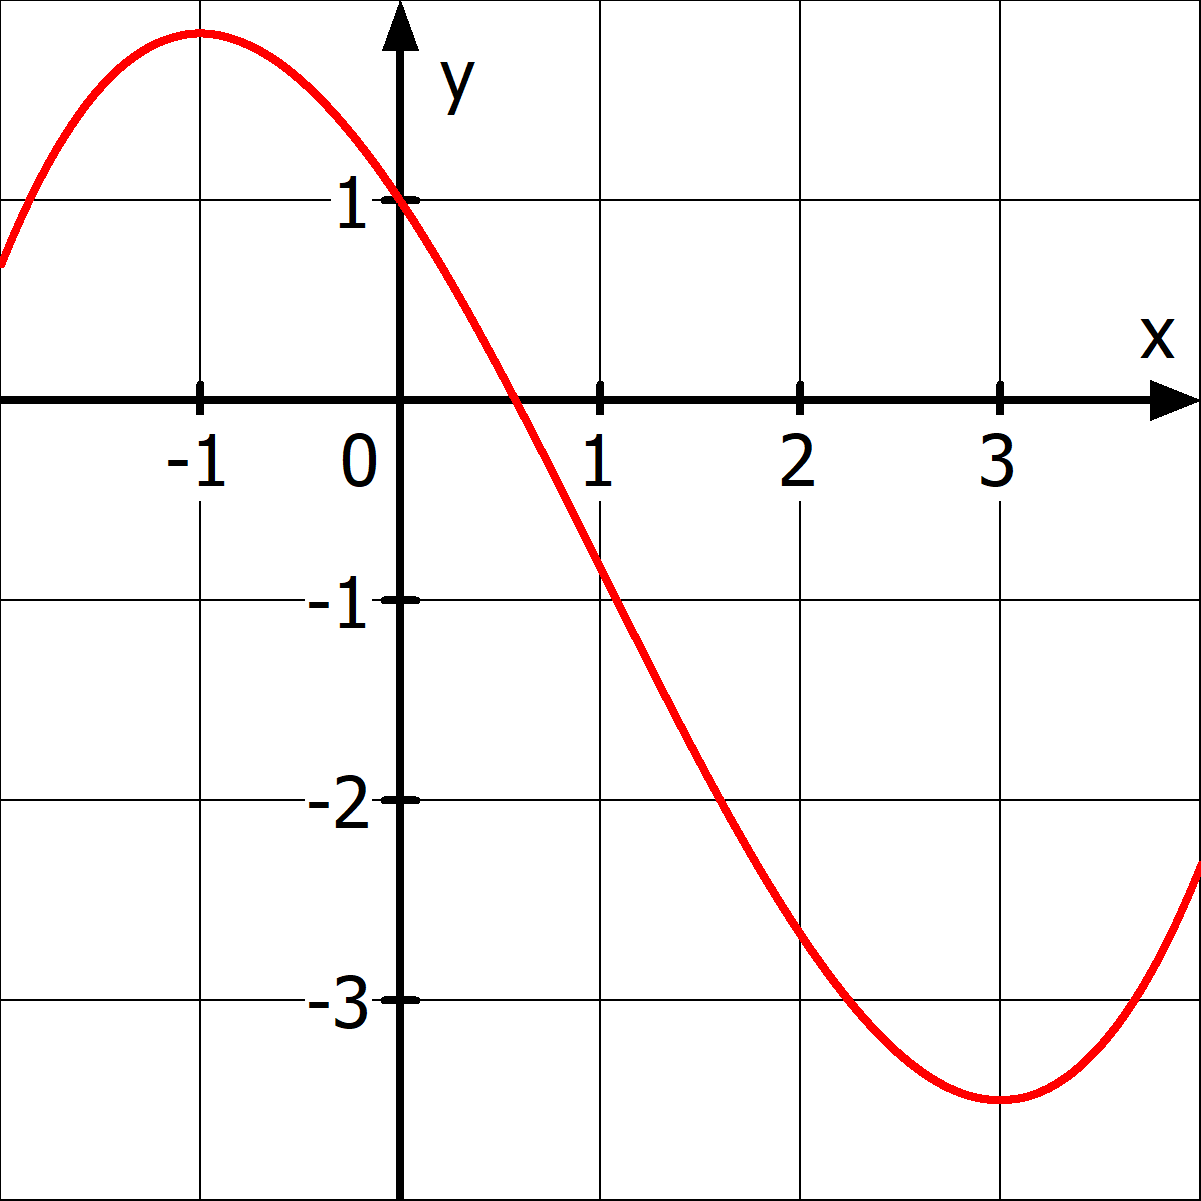
\includegraphics[width=\textwidth]{\ableitung/pics/WP_funktion.png}

			\(f(x)=\frac{1}{6}x^3-\frac{1}{2}x^2-\frac{3}{2}x+1\)

			\textcolor{loes}{Das Schaubild von \(f(x)\) hat bei \(x_0\)=1 einen Wendepunkt.}
	\end{minipage}}%
	\adjustbox{valign=t, padding=1.5ex 0ex 0ex 0ex}{\begin{minipage}{\textwidth/\real{3}-1ex}
			\centering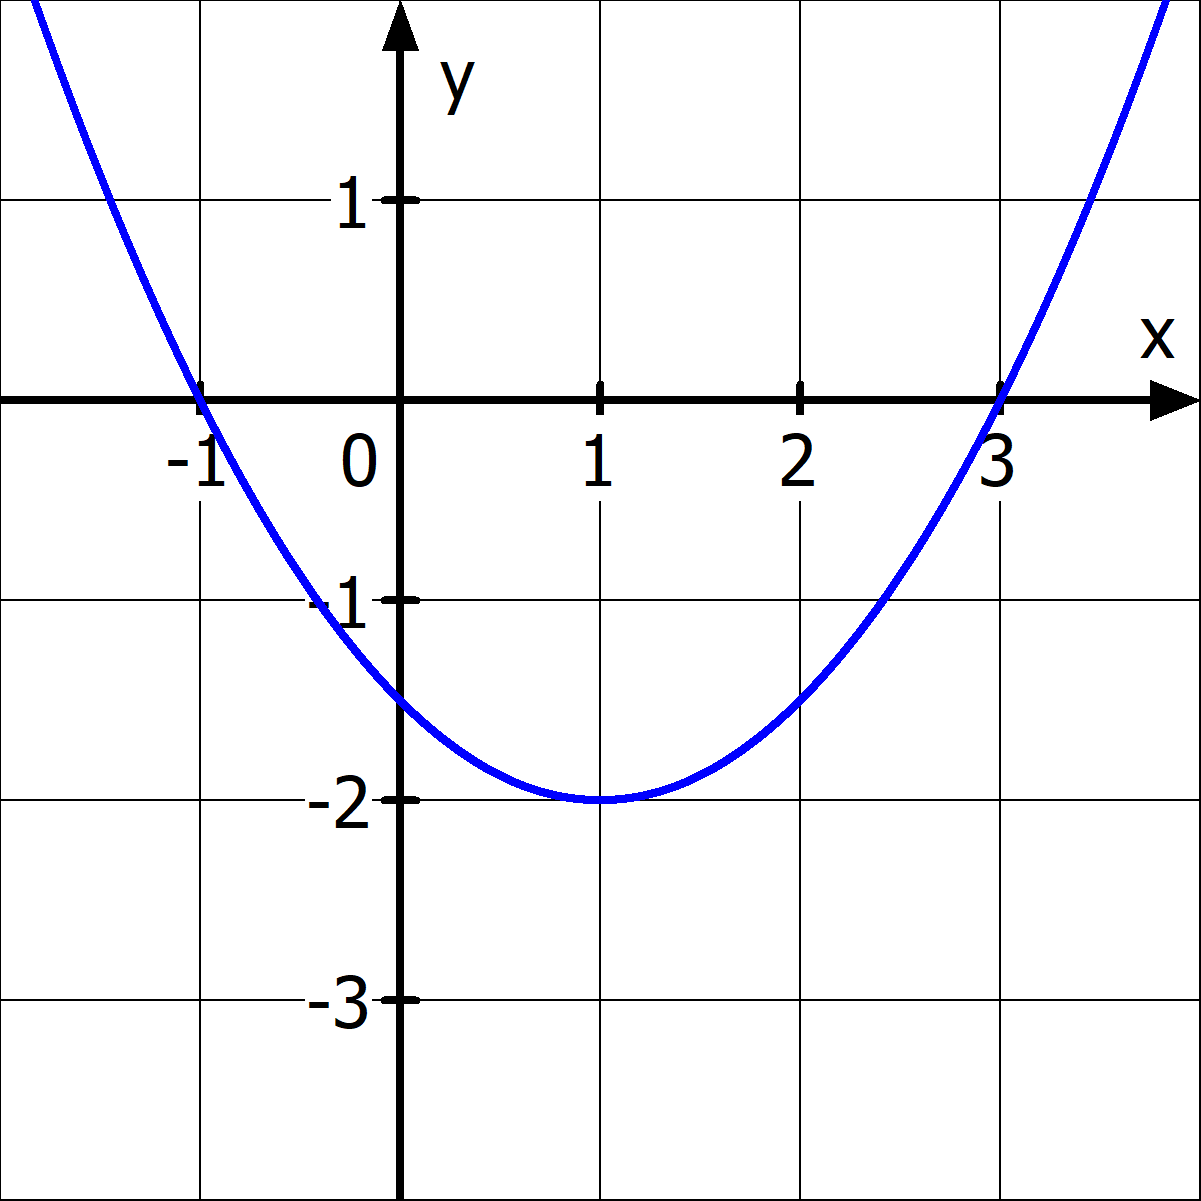
\includegraphics[width=\textwidth]{\ableitung/pics/WP_ableitung.png}

			\(f'(x)=\frac{1}{2}x^2-x-\frac{3}{2}\)

			\textcolor{loes}{Das Schaubild von \(f'(x)\) hat bei \(x_0\)=1 einen Extrempunkt.}
	\end{minipage}}%
	\adjustbox{valign=t, padding=1.5ex 0ex 0ex 0ex}{\begin{minipage}{\textwidth/\real{3}-1ex}
			\centering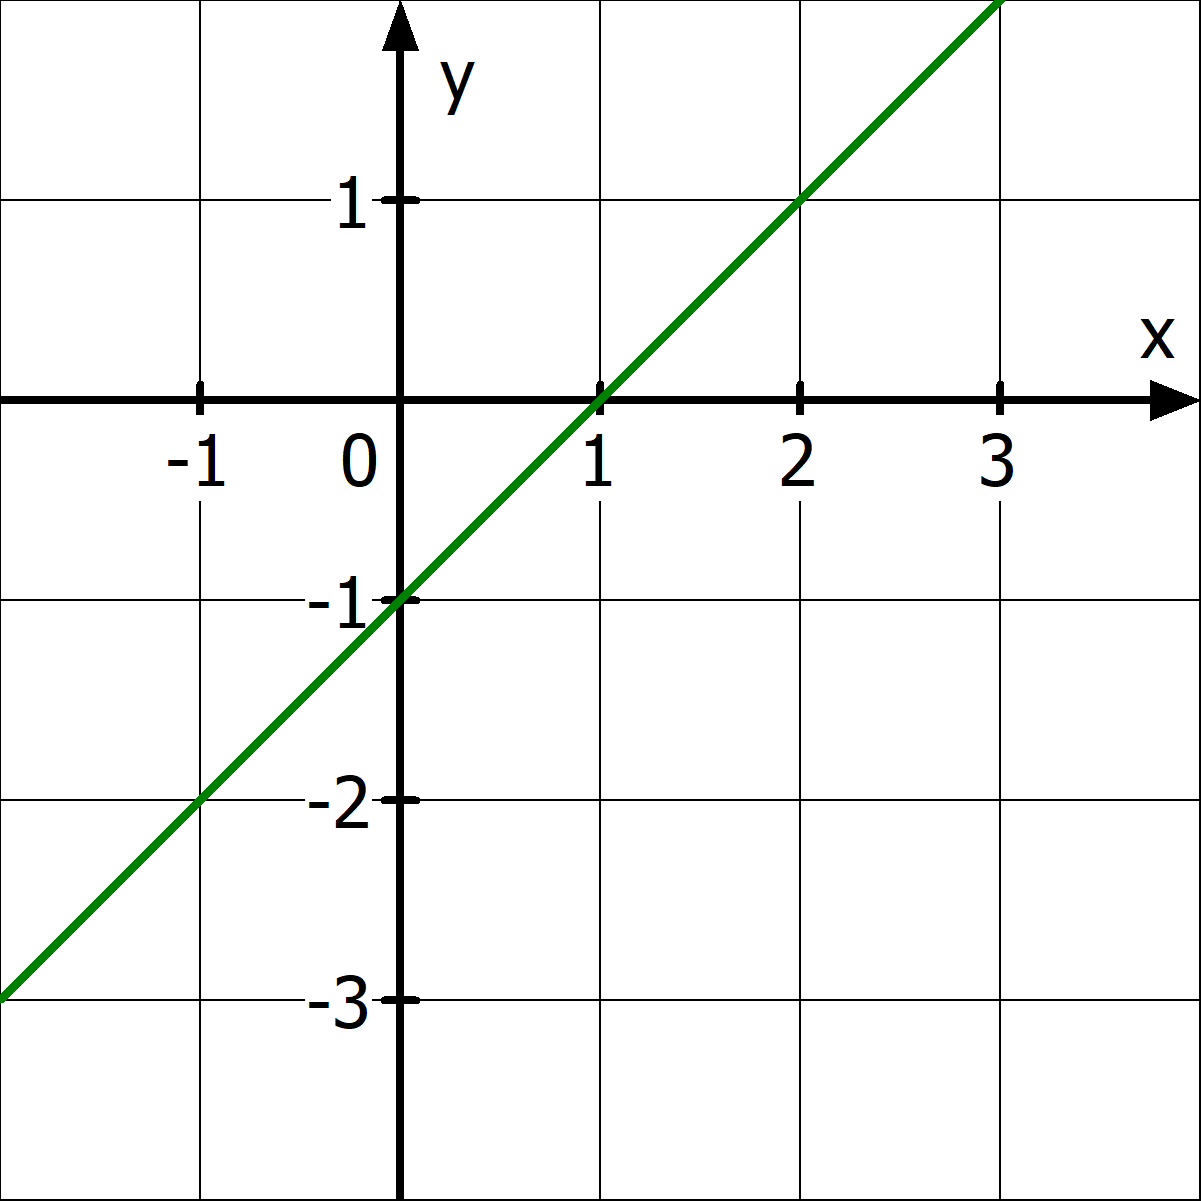
\includegraphics[width=\textwidth]{\ableitung/pics/WP_zwableitung.png}

			\(f''(x)=x-1\)

			\textcolor{loes}{Das Schaubild von \(f''(x)\) hat bei \(x_0\)=1 eine Nullstelle mit Vorzeichenwechsel.}
	\end{minipage}}%
\end{minipage}

\bigskip

\begin{tcolorbox}[width=\textwidth]
    \textbf{Wendetangente:}

    \bigskip

    \textcolor{loestc}{Die Tangente im Wendepunkt nennt man Wendetangente.}

    \bigskip
\end{tcolorbox}

\bigskip

Die Wendetangente im obigen Beispiel berührt das Schaubild im Wendepunkt bei \(W\left(1|f(1)=-\frac{5}{6}\right)\) mit der Steigung \(m_t=f'(1)=-2\). Der \(y\)-Achsenabschnitt ergibt sich aus \(m_t\cdot x_0+b=f(x_0)\)
\begin{align*}
    -2\cdot 1 + b &= -\frac{5}{6}\ \vert+2\\
    b&=\frac{7}{6}
\end{align*}
Die Wendetangente hat also die Gleichung \(t_W(x)=-2x+\frac{7}{6}\)
\newpage
%%%%%%%%%%%%%%%%%%%%%%%%%%%%%%%%%%%%%%%%%%%%%%%%%%%%%%%%%%%%%%%%%%%%%%%%%%%%%%%%%%%%%%%%%%%%%%%%%%%%%%%
\begin{Exercise}[title={\raggedright Bestimme die Wendepunkte.}, label=wendepunkteA1]
	\begin{enumerate}[label=\alph*)]
		\item \(f_1(x)=x^3+3x^2+3x-9\)
		\item \(f_2(x)=0,5x^3-1,5x^2+5\)
		\item \(f_3(x)=-\frac{2}{3}x^3+4x^2-4x-3\)
		\item \(f_4(x)=-\frac{1}{36}x^3+\frac{7}{24}x^2-8x-\frac{55}{144}\)
		\item \(f_5(x)=\frac{5}{12}x^4+\frac{5}{6}x^3-5x^2+x-3\)
		\item \(f_6(x)=-\frac{1}{2}x^4-x^3+\frac{45}{4}x^2+2x-\frac{13}{32}\)
		\item \(f_7(x)=2x^4+16x^3-128x\)
	\end{enumerate}
\end{Exercise}
%%%%%%%%%%%%%%%%%%%%%%%%%%%%%%%%%%%%%%%%%
\begin{Answer}[ref=wendepunkteA1]
	\begin{enumerate}[label=\alph*)]
		\item \(f_1(x):\ W\left(-1\vert -10\right)\)
		\item \(f_2(x):\ W\left(1\vert 4\right)\)
		\item \(f_3(x):\ W\left(2\vert -\frac{1}{3}\right)\)
		\item \(f_4(x):\ W\left(\frac{7}{2}\vert -26\right)\)
		\item \(f_5(x):\ W_1\left(-2\vert -25\right),\ W_2\left(1\vert -\frac{23}{4}\right)\)
		\item \(f_6(x):\ W_1\left(-\frac{5}{2}\vert 61\right),\ W_2\left(\frac{3}{2}\vert 22\right)\)
		\item \(f_7(x):\ W_1\left(0\vert 0\right),\ W_2\left(-4\vert 0\right)\)
	\end{enumerate}
\end{Answer}